\documentclass[11pt,a4 paper]{book}
\usepackage[left=60px, right=60px, bottom=60px, top=60px]{geometry}
\usepackage{amsfonts}
\usepackage{amsmath}
\usepackage{tgtermes}
\usepackage{wrapfig,lipsum,booktabs}
\usepackage{amssymb}
\usepackage{tcolorbox}
\usepackage{titling}
\usepackage{lipsum}
\usepackage{tikz}
\usepackage{xcolor, colortbl}
\usepackage{graphicx}
\usepackage{subcaption}
\usepackage{float}
\usepackage{listings}
\usepackage{setspace}
\usepackage{hyperref}
\usepackage{amsthm}
\usepackage{cases}
\usepackage[utf8]{inputenc}
\usepackage[toc,page]{appendix}
\usepackage{apacite}
\usepackage{siunitx}
\usepackage{url}
\usepackage{sectsty}
\usepackage{listings}
\captionsetup{justification   = raggedleft,
              singlelinecheck = false}
\sectionfont{\color{green!50!black}}\doublespacing
\hypersetup{
    colorlinks,
    linkcolor={blue!90!black},
    citecolor={blue!50!black},
    urlcolor={blue!80!black}
}

\renewcommand\maketitlehooka{\null\mbox{}\vfill}
\renewcommand\maketitlehookd{\vfill\null}
\DeclareMathOperator\arccosh{arcosh}
\theoremstyle{plain}
\newtheorem{thm}{Theorem}[section]
\newtheorem{lem}[thm]{Lemma}
\newtheorem{prop}[thm]{Proposition}
\newtheorem*{cor}{Corollary}
\theoremstyle{definition}
\newtheorem{defn}{Definition}[section]
\newtheorem{conj}{Conjecture}[section]
\newtheorem{exmp}{Example}[section]
\newtheorem{axiom}{Axiom}
\theoremstyle{remark}
\newtheorem*{rem}{Remark}
\newtheorem*{note}{Note}
\renewcommand\maketitlehooka{\null\mbox{}\vfill}
\renewcommand\maketitlehookd{\vfill\null}
\newcommand{\Mod}[1]{\ (\mathrm{mod}\ #1)}

% figure support
\usepackage{import}
\usepackage{xifthen}
\pdfminorversion=7
\usepackage{pdfpages}
\usepackage{transparent}
\newcommand{\incfig}[2][1]{%
\def\svgwidth{#1\columnwidth}
\import{./figures/}{#2.pdf_tex}
}


\begin{document}

\pagenumbering{gobble}
\begin{titlepage}
\begin{center}
\large
University of Warwick \\
Department of Computer Science \\
\huge
\vspace{50mm}
\rule{\linewidth}{0.5pt} \\
CS118 \\
\vspace{5mm}
\Large
Programming for Computer Scientists
\rule{\linewidth}{0.5pt}
\vspace{5mm}
\begin{figure}[H]
\centering
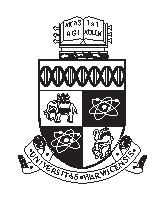
\includegraphics[width=0.4\textwidth]{crest_black.eps}
\end{figure}
\vspace{37mm}
Cem Yilmaz\\
\today
\end{center}
\end{titlepage}
\newpage
\tableofcontents
\newpage
\pagenumbering{arabic}
\setcounter{page}{1}
\begin{flushleft}
\chapter{Definitions}
\begin{defn}Binary is the representation used by computers in a base $2$ number system. It is represented by two numbers, $0$ and $1$.
\end{defn}
\begin{defn}
Bits is the digit size for the binary system.
\end{defn}
\begin{defn}
Byte is 8 bits, aka 8 digits in base $2$.
\end{defn}
\begin{defn}
Function in computer science is the command which tells the computer to execute something. It is an action or a verb.
\end{defn}
\begin{defn}
Conditions in computer science gives the choice to the computer to do an action depending on what is present. e.g. if or else statement
\end{defn}
\begin{defn}
Loop in computer science is the command that returns the computer to a specific line to repeat programs
\end{defn}
\begin{defn}
A boolean question is a question whose answer is yes or no. They are usually paired with conditions.
\end{defn}
\begin{defn}
A string is characters sandwiched between quotation marks.
\end{defn}
\begin{defn}
A statement terminator is a semi-colon (;), and it ends statements. Every statement in Java must be terminated. 
\end{defn}
\begin{defn}
An interpreter reads one statement from the source code, translates it to the machine 
code or virtual machine code, then executes it.
\end{defn}
\begin{defn}
A compiler fully translates all of the source code into machine code for execution.
\end{defn}
\begin{defn}
Casting is an operation that converts the value of one data type into a value of another data type.
\end{defn}
\chapter{Base $n$ counting}
\section{Binary}
\subsection{The connection between between Base $2$ and Base $10$}
Counting is the same no matter base system one uses, just represented differently. In Base $10$, when we reach from $0$ to $9$ and add $+1$, we add a tens digit to represent higher numbers. In Base $2$, a similar system follows, however, instead for counting from $0$ to $9$, we do it with $0$ and $1$. For example, let us consider the numbers $123$. It can also be represented as
\begin{align}
&\underbrace{1}_{1 \times 10^2}\underbrace{2}_{2 \times 10^1}\underbrace{3}_{3 \times 10^0}\\
\implies &1\times10^2+2\times10^1+3\times10^0
\end{align}
Generalisation for a number of $n$ digits
\begin{align}
abc,def,\ldots \zeta \\
\underbrace{a}_{a \times 10^n}\underbrace{b}_{b\times 10^{n-1}}\underbrace{c}_{c \times 10^{n-2}},\underbrace{d}_{d \times 10^{n-3}}\underbrace{e}_{e \times 10^{n-4}} \underbrace{f}_{f \times 10^{n-5}},\ldots \underbrace{\zeta}_{\zeta\times 10^0}
\end{align}
The coefficient $b$ in a base 10 for a digit $a10^{n+1}+b10^n$ can be any of the numbers $a,b \in \{0,1,2,\cdots,9\}$, as when it goes above $9$, it will add an extra $1$ to $a$, i.e. it will become 
\begin{align}
a10^{n+1}+(b+10)10^n \iff (a+1)10^{n+1}+b10^n
\end{align}
In base $2$, a similar principle follows. Let us consider a few numbers
\begin{align}
0 \implies 0 \text{ base } 10\\
1 \implies 1 \text{ base } 10\\
10 \implies 2 \text { base } 10 \\
11 \implies 3 \text { base } 10 \\
100 \implies 4 \text { base } 10 \\
101 \implies 5 \text { base } 10
\end{align}
It is possible to see that for each new digit added, instead of growing with $10^n$, we grow as $2^n$ for $n$ binaries digits (bits). Furthermore, our coefficient for each digit must either be $0$ or $1$, meaning that the power $2^n$ exists or it doesn't. Hence, we actually count for $a,b,\zeta \in \{0,1\}$
\begin{align}
a2^n+b2^{n-1}+\cdots+\zeta 2^0
\end{align}
We can convert a number from base $2$ to base $10$ using the formula above. Similarly,
\begin{align}
a2^{n+1}+(b+2)2^n \iff (a+1)2^{n+1}+b2^n
\end{align}
\subsection{Base $n$}
Hence we can generalise further, for base $n$ counting we have the following rules with coefficients $a,b,\zeta \in \{0,1,\ldots,n-1\}$ and an $\alpha$ digit number in base $n$:
\begin{align}
an^{\alpha}+bn^{\alpha-1}+\cdots+\zeta n^0
\end{align}
and
\begin{align}
an^{\alpha+1}+(b+n)n^\alpha \iff (a+1)n^{\alpha+1}+bn^\alpha
\end{align}
\chapter{Understanding Java}
Java is a programming language that can be run in many OS thanks to JVM (Java Virtual Machine). This allows for it to run "bytecode" within any operating system. When a .java program is launched, the java file is compiled into bytecode with a .class file extension. This bytecode is then interpreted by JVM and is finally translated into binary. The figures below represent the hierarchy of the execution of Java code.
\begin{figure}[H]
\centering
\makebox[\textwidth][c]{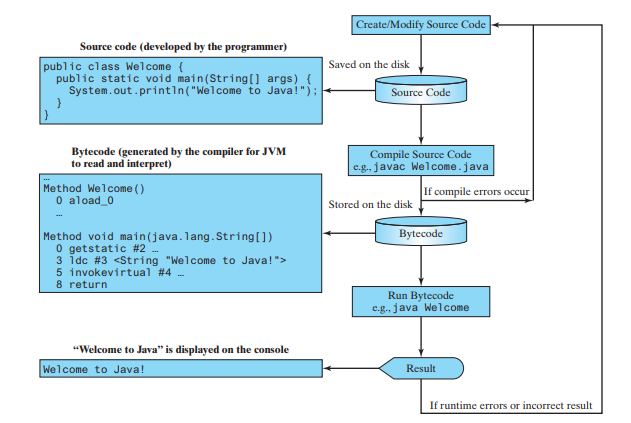
\includegraphics[scale=1]{compile.png}}

\caption{The execution cycle of a java program}
\label{fig:cycle}
\end{figure}
\newpage
Furthermore, there is a difference between a compiler and an interpreter for an IDE
\begin{figure}[H]
\centering
\makebox[\textwidth][c]{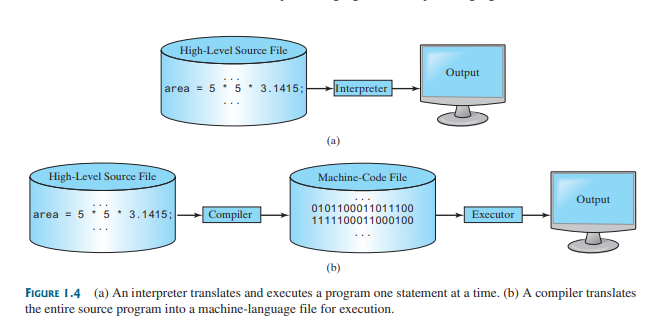
\includegraphics[scale=0.8]{interpreter.png}}
\label{fig:cycle}
\end{figure}
\section{Errors}
\subsection{Syntax Error}
Errors which are detectable by the compiler are called syntax or compile errors. These are caused when a code is constructed wrongly, e.g. mistyping, missing punctuation, brace etc.
\subsection{Runtime Error}
In runtime errors, a program terminates abnormally. This happens because the program expects a certain value but the user inserts a value that the program is not able to handle. E.g. if there is an expectation of a number but there is a string.
\subsection{Logic Error}
Occurs when a program does not output what it is intended to output. E.g. integer division using floor function to output the final answer
\section{Variables}
A variable represents a value stored in the computer’s memory. Variables which are defined by their data type, on example of which is $double$.
\begin{figure}[H]
\centering
\makebox[\textwidth][c]{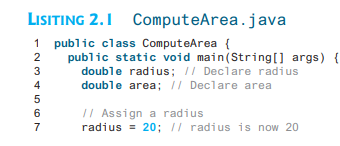
\includegraphics[scale=0.8]{double.png}}
\label{fig:double}
\caption{Use of double to define radius and area}
\end{figure} 
This can be used to create shortcuts. Furthermore, in strings, the $+$ sign can also be used as the string concatenation operator. In other words, it can also be used to combine strings. For example,
\begin{figure}[H]
\centering
\makebox[\textwidth][c]{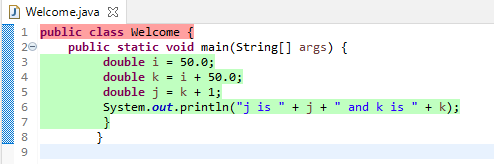
\includegraphics[scale=0.8]{exxample.png}}
\label{fig:example1}
\caption{Use of double and $+$ as a concatenation operator}
\end{figure} 
\section{Taking in input from console}
Suppose that now we want to change the definition of radius to another number. For an input, the way we have defined print is to be $System.out$. however, for input, our new command is $System.in$. To perform console input, you need to use the Scanner class to create an object to read input from System.in, as follows:
\begin{lstlisting}[language = Java]
Scanner input = new Scanner(System.in);
\end{lstlisting}
The syntax new Scanner(System.in) creates an object of the Scanner type. The syntax Scanner input declares that input is a variable whose type is Scanner. The whole line Scanner input = new Scanner(System.in) creates a Scanner object and assigns its reference to the variable input. An object may invoke its methods. To invoke a method on an object is to ask the object to perform a task. You can invoke the nextDouble() method to read a double value as follows:
\begin{lstlisting}[language = Java]
double radius = input.nextDouble();
\end{lstlisting}
This statement reads a number from the keyboard and assigns the number to radius. We could also have several of these statements together separated by a line, and we would be able input all of these in a single line. That is:

\begin{figure}[H]
\centering
\makebox[\textwidth][c]{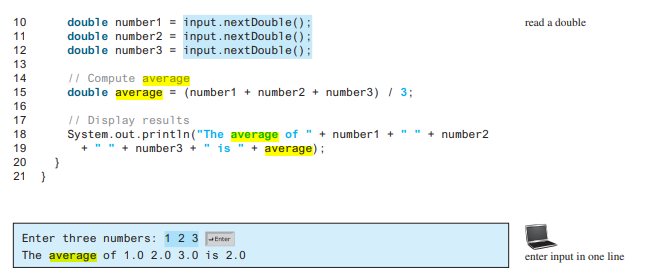
\includegraphics[scale=1]{input.png}}
\label{fig:input}
\caption{Three inputs demonstration}
\end{figure} 
 However, for this to work, we require the package Scanner which is obtained by writing
\begin{lstlisting}[language= Java]
import java.util.Scanner; // Scanner is in the java.util package
\end{lstlisting}
The code above only imports Scanner from the java.util package. This is a specific imports. We could've also replaced .Scanner with .* which would  then turn it into a wildcard import, that is, it would import everything in the package. There is no performance difference between the two. For now, also simply accept that is how objects are declared to create inputs.
\section{Identifiers}
Identifiers are the names that identify the elements such as classes, methods, and variables in a program. For example, the program name "Welcome" is an identifier. radius and area are identifiers. Main and input are also identifiers. All identifiers must obey the following rules:
\begin{enumerate}
\item An identifier is a sequence of characters that consists of letters, digits, underscores (\_), and dollar signs (\$).
\item An identifier must start with a letter, an underscore (\_), or a dollar sign (\$). It cannot start with a digit.
\item An identifier cannot be a reserved word.
\item An identifier cannot be true, false, or null.
\item An identifier can be of any length.
\end{enumerate}
\section{Variables and Data Types}
Variables are used to store certain information using an identifier. They can be declared by doing
\begin{lstlisting}[language=Java]
datatype VariableName;
\end{lstlisting}
The datatypes that exist are the following:
\begin{lstlisting}[language=Java]
double //used to denote a real number to 15 decimal points 
int //used to denote an integer from -2,147,483,648 to 2,147,483,647
boolean // used to denote true or false
byte // used to store integer numbers from -128 to 127
short // stores whole numbers from -32,678 to 32,767
long // Stores whole numbers from -9,223,372,036,854,775,808 
// to 9,223,372,036,854,775,807
float // Stores a real number to 7 decimal points
\end{lstlisting}
\begin{figure}[H]
\centering
\makebox[\textwidth][c]{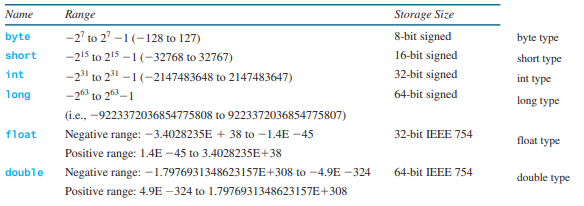
\includegraphics[scale=1]{data type.png}}
\label{fig:datatypes}
\end{figure} 
\begin{figure}[H]
	\centering
	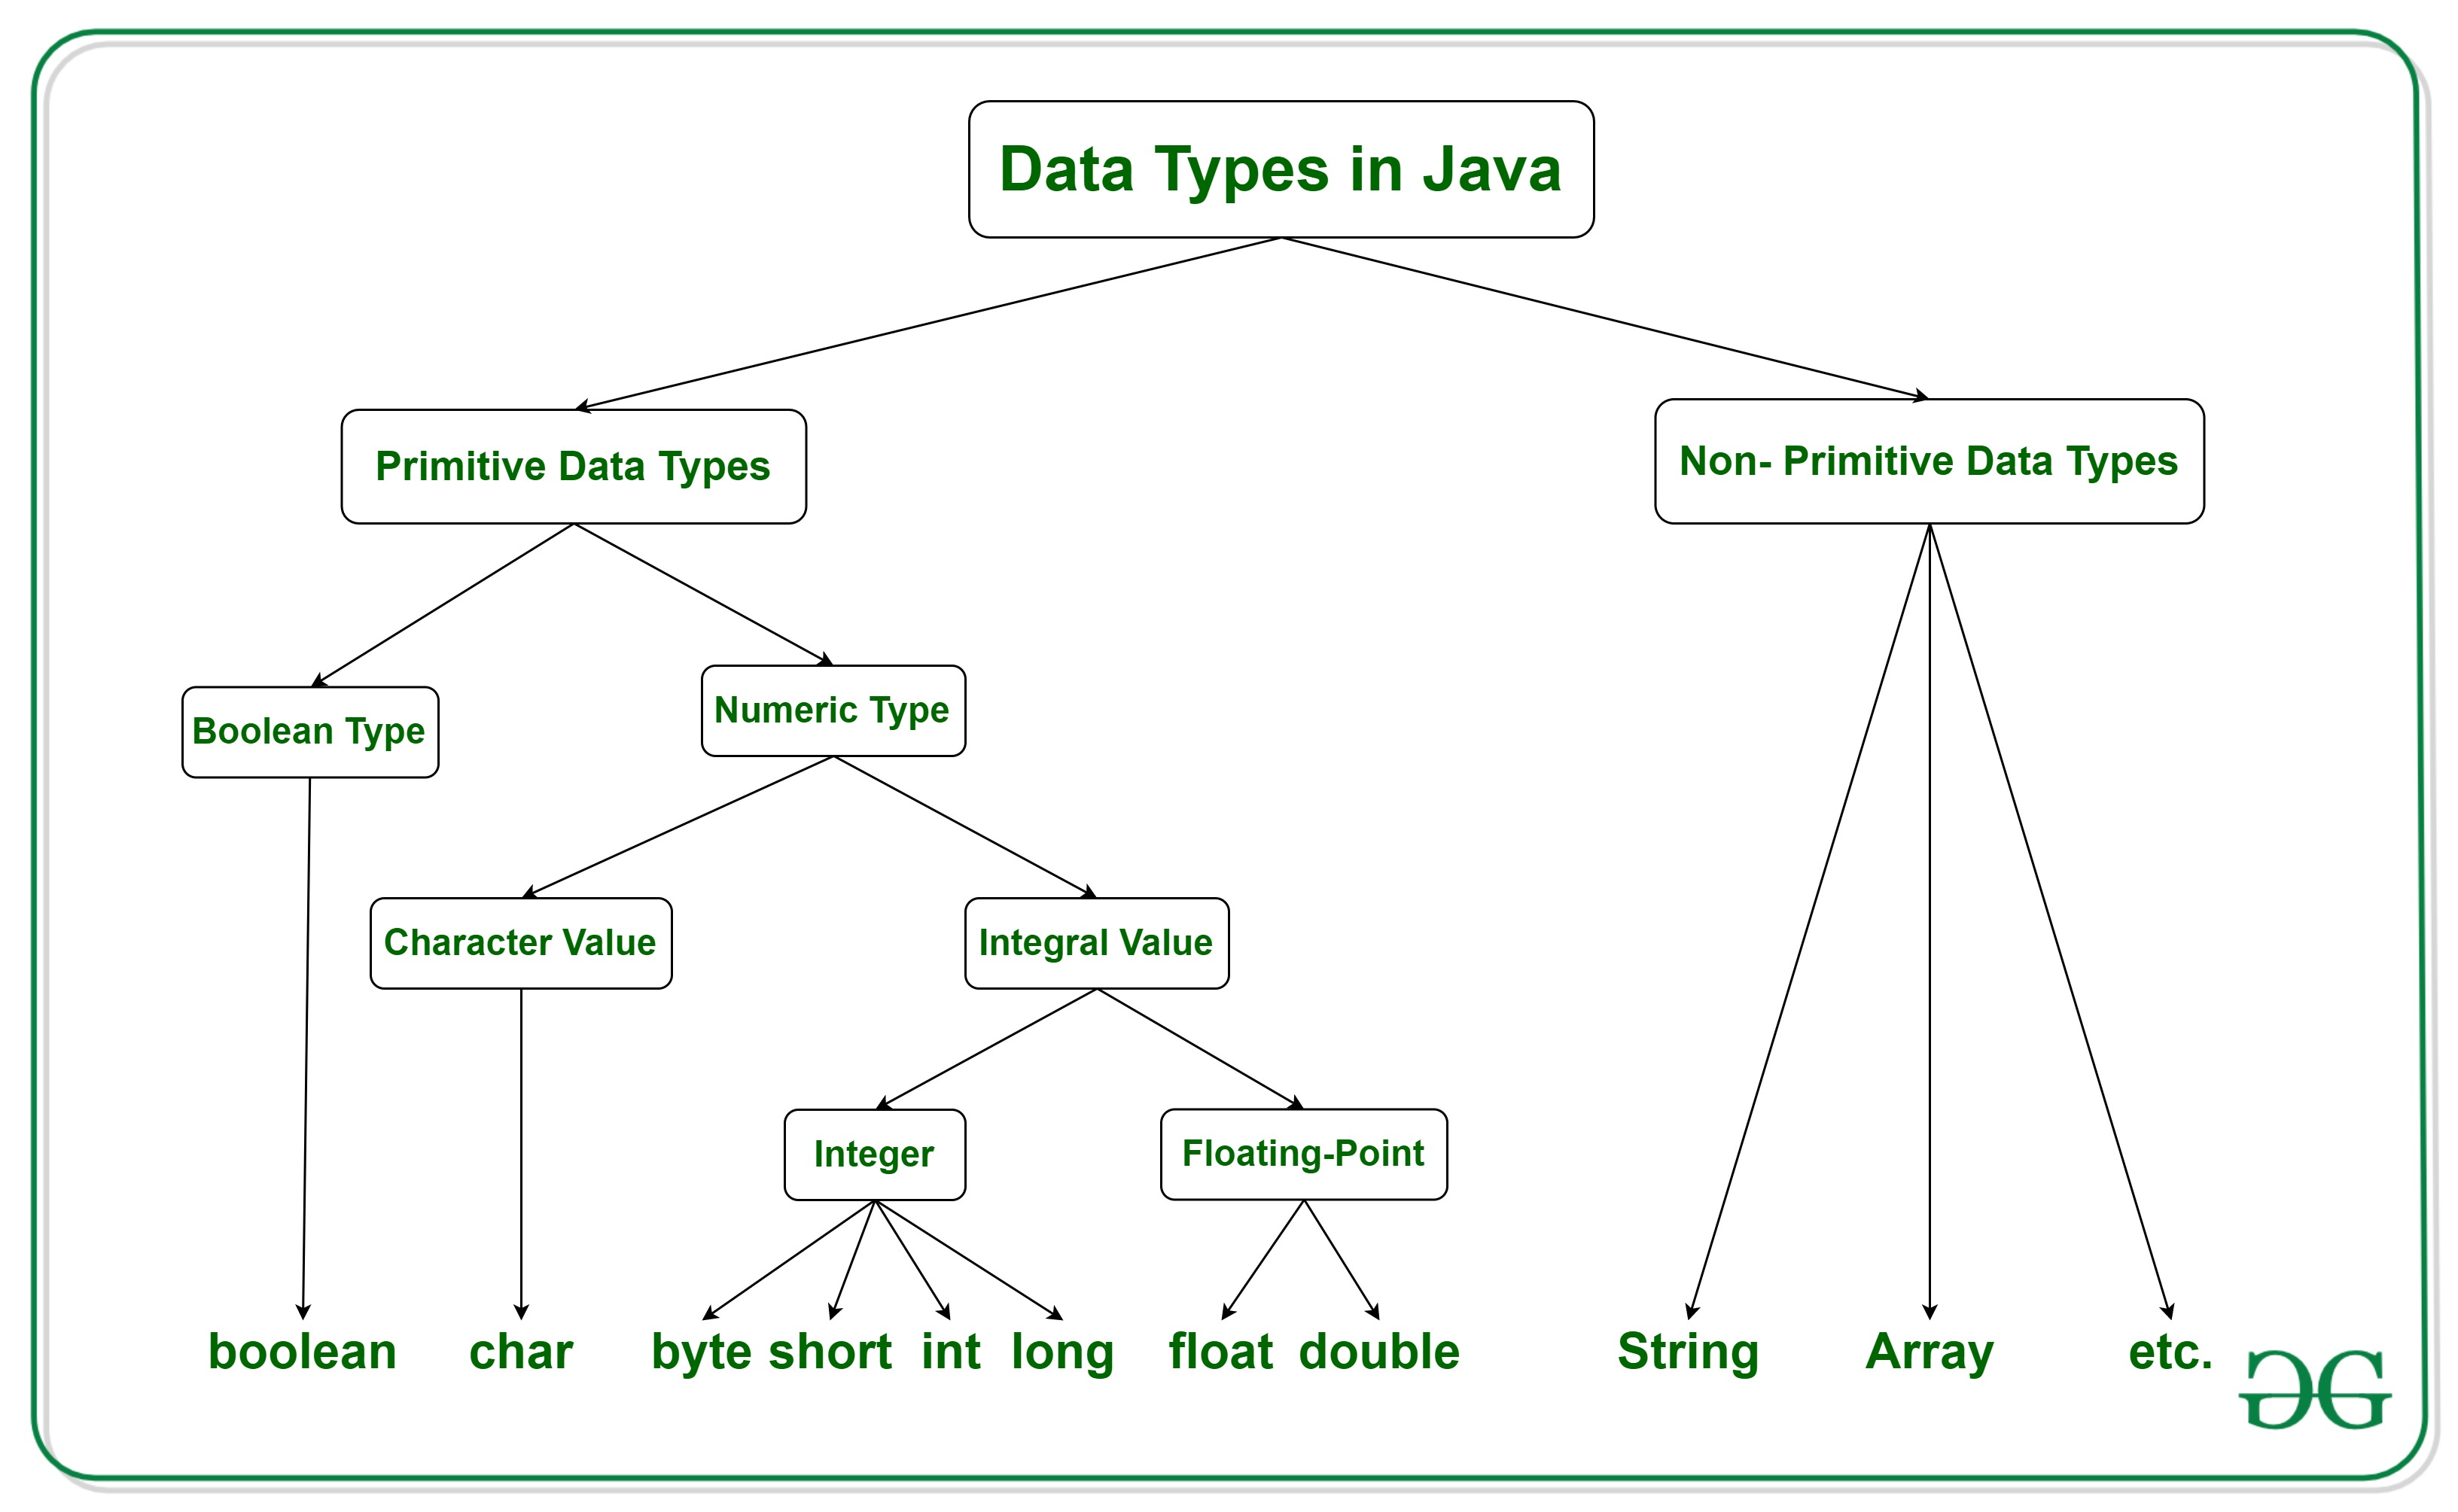
\includegraphics[width=0.8\textwidth]{data.png}
	\caption{Data types}
	\label{fig:data-png}
\end{figure}
\begin{tcolorbox}[colback=black!3!white,colframe=black!60!white,title=\begin{defn}How Number range is determined \label{How Number range is determined}\end{defn}]
It is important to understand why, for example, in a byte it counts from $-2^{7}$ to $2^{7}-1$.
From definition, we know that a byte is 8 bits, that is, $00000000$. The biggest number, we can get, is therefore $11111111$, which translates to $255$. However, we also need to define the negative numbers, and this was done by definition by setting the most left number $1 $. That is, $10000000$ is in fact $-128$. The rest of the zeroes are computed as $-128+a$, where $a$ is determined by the $0000000$. For example, $10000001$ is $-127$. This means the highest positive integer we can achieve is  $01111111$, which is $127$. 
\end{tcolorbox}
NOTE: it is important that for float values and that for long values, we must put L at the end of a number if it the number goes beyond integer's limits. Similarly, to declare a float value, it is recommended to put an F.
The biggest difference between datatypes are their data that takes it to store. For example, double is 8 bytes whereas float is 4 bytes. Furthermore, if a datatype is a constant, then you can add the $final$ text beforehand declaring the variable. This declares that it is a constant with unchanging data. By convention, constants are also written with capital letters. For example
\begin{lstlisting}[language=Java]
final double PI = 3.14159;
\end{lstlisting}
\section{Math operators}
Other than adding, subtracting, multiplying and dividing, we also have the remainder and the exponent math operators in Java. They are declared as the following:
\begin{lstlisting}[language=Java]
% // This is the remainder operator. For example, 5 % 3 would give out 2.
Math.pow(a, b)// This is the power operator. This would show a^b.
\end{lstlisting}
\section{Number Literals}
\section{Augmented Assignment Operators}
The operators +, -, *, /, and \% can be combined with the assignment operator to form augmented operators.
For example, we can define $x=x+1$, this way, the variable $x$ increases by $1$. These augmented assignments also have shortcuts, which are shown in the table below:
\begin{figure}[H]
\centering
\makebox[\textwidth][c]{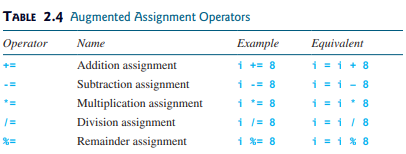
\includegraphics[scale=1]{aao.png}}
\label{fig:aao}
\end{figure} 
\section{Increment and Decrement operators}
\begin{figure}[H]
\centering
\makebox[\textwidth][c]{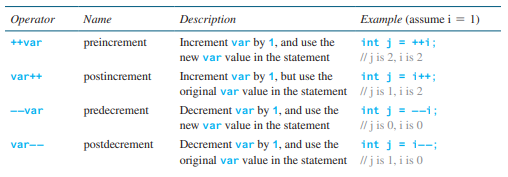
\includegraphics[scale=1]{ido.png}}
\label{fig:ido}
\end{figure} 
\section{Numeric Type Conversions}
In Java, widening cast type will be automatically done. However, narrowing cast will require manual work.   The type of data type for a number can be expressed by adding 
\begin{lstlisting}[language=Java]
(Data type)Number
\end{lstlisting}
That is, for example
\begin{lstlisting}[language=Java]
public class Example {
	public static void main(String[] args) {
		System.out.println(1/2);
		// this will display zero because the output will originally
		// display 0.5 with floor function 0.
		System.out.println((double)1 / 2) 
		// this will display 0.5 due to the double operator.
	}
}
\end{lstlisting}
\section{Software Development Process}
\begin{figure}[H]
\centering
\makebox[\textwidth][c]{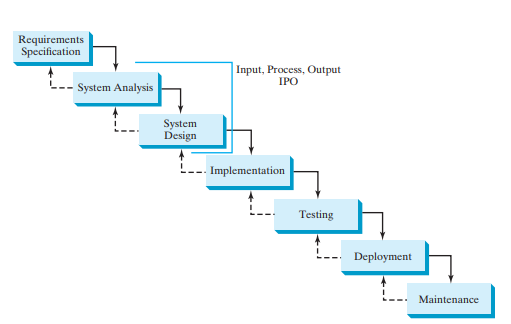
\includegraphics[scale=0.8]{sdp.png}}
\label{fig:example1}
\caption{Software Development Process visualised}
\end{figure} 
\begin{enumerate}
\item Requirements specification - seek and understand the problem the software will address. It will also require documentation of what the software system needs to do.
\item System analysis - identify the system's input and output. It is easier to find the output first, and then base off inputs depending on the output.
\item System Design - a process for obtaining the output from the input. This phase 
involves the use of many levels of abstraction to break down the problem into manageable 
components and design strategies for implementing each component. 
\item Implementation - bringing the project to life by writing code as planned in system design. Separate programs are written for each component then integrated together.
\item Testing - ensure that the code written is functional in different scenarios. 
\item Deployment - how the software will be distributed to the public, e.g. installation or server online
\item Maintenance - updating and improving the product after launch. If the software is planned to be lasting, then it must be periodically upgraded.
\end{enumerate}
\chapter{Selections}
In this chapter we will look into choosing alternative courses depending on the input.
\section{Boolean Data Types}
Boolean data types allow us to compare the numerical input to desired limits. The table below shows an example of these data types. Assume that the radius of the circle is $10$.
\begin{figure}[H]
\centering
\makebox[\textwidth][c]{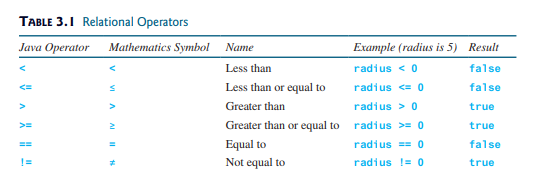
\includegraphics[scale=0.8]{booleandata.png}}
\label{fig:booleandata}
\caption{Table of Boolean Data Types}
\end{figure} 
A boolean value is always true or false. We could, for example, assign a true or false value a variable. 
\begin{lstlisting}[language=Java]
boolean lightsOn = true;
\end{lstlisting}
\section{if Statements}
\subsection{one-way if statements}
Java has several types of selection statements: one-way if statements, two-way if-else
statements, nested if statements, multi-way if-else statements, switch statements, and 
conditional operators.
A one-way if statement executes an action if and only if the condition is true. The syntax 
for a one-way if statement is as follows:
\begin{lstlisting}[language=Java]
if (boolean-expression) {
statement(s);
}
\end{lstlisting}
In other words,
\begin{figure}[H]
\centering
\makebox[\textwidth][c]{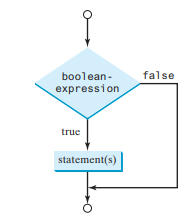
\includegraphics[scale=0.8]{st.png}}
\label{fig:st}
\caption{If expression flowchart}

\end{figure} 
However, note that the brackets $\{\}$ are not necessarily required if the statement is 1 line only.
\subsection{Two-Way if statements}
A two-way if statement considers another statement if the answer to the if statement is false.
\begin{lstlisting}[language=Java]
if (boolean-expression) {
 statement(s)-for-the-true-case;
}
else {
 statement(s)-for-the-false-case;
} 
\end{lstlisting}
\subsection{Nested and Multi-way if and if-else statements}
A nested if statement is defined that if the statement for either the true case or the false case contains another if or if else statement. 
A good example of a nested and multi-way statement is the following:
\begin{lstlisting}[language=Java]
if (score >= 90)
 System.out.print("A");
else if (score >= 80)
 System.out.print("B");
else if (score >= 70)
 System.out.print("C");
else if (score >= 60)
 System.out.print("D"); 
else
 System.out.print("F");
\end{lstlisting}
However, it is important to see that this code works because it keeps introducing a new range for checking. Consider the following code, which is blatantly wrong:
\begin{lstlisting}[language=Java]
if (score >= 60)
 System.out.println("D");
else if (score >= 70)
 System.out.println("C");
else if (score >= 80)
 System.out.println("B");
else if (score >= 90)
 System.out.println("A");
else
 System.out.println("F");
\end{lstlisting}
\subsection{Common and crucial errors}
\subsubsection{Math float points}
Unfortunately, because numbers in computer science definitions aren't precise, things can get messy. Consider the following code:
\begin{lstlisting}[language=Java]
double x = 1.0 - 0.1 - 0.1 - 0.1 - 0.1 - 0.1;
System.out.println(x == 0.5);
\end{lstlisting}
And this is in fact false. The final value of $x$ is around $x=0.5000000000000001$. One way to avoid this, is to introduce the variable $\varepsilon$, a small number that will allow us to create comparisons. That is, we can check if it is sufficiently close enough by computing $|x-y|<\varepsilon$.  Normally, you set e
to $1E-14$ for comparing two values of the double type, and to $1E-7$ for comparing two values of the float type. For example:
\begin{lstlisting}[language=Java]
final double EPSILON = 1E-14;
double x = 1.0 - 0.1 - 0.1 - 0.1 - 0.1 - 0.1;
if (Math.abs(x - 0.5) < EPSILON)
 System.out.println(x + " is approximately 0.5");
 \end{lstlisting}
 \subsubsection{Boolean operator assignment}
Do not use the if statement to create assignment values for boolean when it can be simplified by denoting the boolean variable in the first place. Consider the following example:
\begin{lstlisting}[language=Java]
if (number % 2 == 0)
even = true;
else
even = false;
\end{lstlisting}
It could instead be written better as 
\begin{lstlisting}[language=Java]
boolean even = number % 2 == 0;
\end{lstlisting}
\subsection{Random Number Generator}
A good approach to generate randoms is to utilise the random from Math class. It generates a random number $d$ such that $0 \leq d < 1$. 
\subsection{Logical Operators}
\begin{figure}[H]
\centering
\makebox[\textwidth][c]{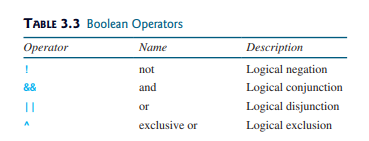
\includegraphics[scale=1]{operator.png}}
\label{fig:input}
\caption{Logical operators}
\end{figure} 
These apply operators work as the following:
\begin{table}[H]
	\centering
	\caption{! NOT operator}
	\label{tab:NOT}
	\begin{tabular}{ccc}
		\hline
		Value 1 & Output \\
		\hline
		T	&	F\\
		F	&	T \\
		\hline
	\end{tabular}
\end{table}
\begin{table}[H]
	\centering
	\caption{AND operator}
	\label{tab:and}
	\begin{tabular}{ccc}
		\hline
		Value 1 & Value 2 & Output \\
		\hline
		T	& T	  & T \\
		T	& F	  & F \\ F	& T	  & F \\ F	& F	  & F \\ \hline \end{tabular} \end{table} \begin{table}[H]
	\centering
	\caption{OR operator}
	\label{tab:OR}
	\begin{tabular}{ccc}
		\hline
	Value 1 & Value 2 & Output \\
	\hline
	T	& T	  & T \\
	T	& F	  & T \\
	F	& T	  & T \\
	F	& F	  & F \\
	\hline
	\end{tabular}
\end{table}
\begin{table}[H]
	\centering
	\caption{XOR operator}
	\label{tab:XOR}
	\begin{tabular}{ccc}
		\hline
	Value 1 & Value 2 & Output \\
	\hline
	T & T & F \\
	T & F & T \\
	F & T & T \\
	F & F & F \\
	\hline
	\end{tabular}
\end{table}
However, it is important to note that for the AND and the OR statement listed above, if the first is true, it will NOT check the second case.
\begin{tcolorbox}[colback=black!3!white,colframe=black!60!white,title=\begin{thm}De Morgan's Law \label{De Morgan's Law}\end{thm}]
	De Morgan's Law states specific rules for boolean logic algebra. Before the math is invoked below, it is important to know that these are the notations: \\	
	NOT: $\neg = !$ \\
	AND: $\land = \string& \string& $ \\
	OR: $\lor =  \mid\mid $ \\
	XOR (Exclusive): $\oplus = \string^$ \\
	Logical Equivalence: $\equiv$ \\
	Material Conditional:  $\to $

		\begin{align}
			\neg\left( A \land B \right) \equiv \neg A \lor \neg B\\
			\neg\left( A \lor B \right) \equiv \neg A \land \neg B 
		\end{align}

\end{tcolorbox} 
Other rules of Boolean algebra include but are not limited to the following:
\begin{align*}
	\neg\left( A \oplus B\right) = A \equiv B
\end{align*}
Material conditional is always true except when $A$ is false and $B$ is true.

\subsection{switch Statements}
A cumulation of if statements can be avoided with the creation of a switch statement. A switch statements will run onto a specific line depending on the case that is in the input. An example can be seen below:
\begin{lstlisting}[language = Java]
switch (status) {
	case 0: statement(s)-for-case-0;
		break;
	case 1: statement(s)-for-case-1;
		break;
	case 2: statement(s)-for-case-2;
		break;
	case 3: statement(s)-for-case-3;
		break;
	default:statement(s)-for-default;
		System.exit(1);
	}
\end{lstlisting}
The only thing to keep note here is that the case number $n$ must be the same data type.

\subsection{Conditional Operators}
Conditional operator is used to assign a variable depending on whether the boolean expression is true or not. Namely:
\begin{lstlisting}[language = Java]
y = (x > 0) ? 1 : -1;
\end{lstlisting}
This is equivalent to
\begin{lstlisting}[language = Java]
if (x > 0)
 y=1;
else
 y=-1;
\end{lstlisting}
\subsection{Operator Precedence and Associativity}
\begin{table}[H]
	\centering
	\caption{Precedence and Associativity}
	\label{tab:PaA}
	\begin{tabular}{cc}
	0 & $var++$ and $var--$ \\
	1 & $+,-$ (Unary plus and minus), $++var,--var$ \\
	2 & $!$ (Not) \\
	3 & $*,\string/, \%$ \\
	4 & $+,-$ (Binary addition and subtraction) \\
	5 & $<,<=,>,>=$ \\
	6 & $==, != $ \\
	7 & $\string^$ \\
	8 &  $\&\&$ \\
	9 & $ \mid  \mid $ \\
	10 & $=,+=,-=.*=,\string/=,\%=$
	\end{tabular}
\end{table}
Where the smaller the number, the higher the priority.
Another important thing to note is the associativity of these. It follows that for regular operators the associativity goes from left to right. That is, if the priority is the same. The output is calculated by going from left to right. However, assignment operators, e.g. $+=,=$ etc. are right associative.
\subsection{Debugging}
Logical errors are called bugs. Debugging is the process of finding these logical errors. Methods of debugging, which are usually integrated to the idea, are the following:
\begin{enumerate}
	\item Executing a single statement at a time - The debugger allows you to execute one statement at a time to see the effect of each statement
	\item Tracing into or stepping over a method - You can skip over some methods. For example, you would always step over system-applied methods e.g. System.out.println();
	\item Setting breakpoints - Your program pauses at this breakpoint. You can set as many of these as you want.
	\item Displaying variables - The debugger allows you to select variables and display their values.
	\item Displaying call stacks - The dubber allows you to trace all of the method calls. 
	\item Modifying variables - Some debuggers enable you to modify the value of a variable when debugging for testing.
\end{enumerate}
\section{Mathematical Functions, Characters, and String}
\subsection{Mathematical Functions}
All math functions in Java are executed by first writing $Math.$, followed by the function itself. There are many such functions, including, but not limited to:
\begin{lstlisting}[language = Java]
Math.sin();
Math.cos();
Math.tan();
Math.toRadians();
Math.toDegrees();
Math.asin();
Math.acos();
Math.atan();
\end{lstlisting}
However, note that this is all done in Radians by default. Other useful constants include $PI$ and $E$ which are $\pi$ and $e$ respectively. For exponents, the list is the following:
\begin{lstlisting}[language = Java]
Math.exp();
log();
log10();
pow(a, b);
sqrt();
\end{lstlisting}
Finally, we can also use math to round numbers
\begin{lstlisting}[language = Java]
ceil();
floor();
rint();
round(); // Returns (int)Math.floor(x + 0.5) if x is float and returns
// (long)Math.floor(x+0.5) if x is double. 
\end{lstlisting}
\subsection{Data Type and Operations}
\subsubsection{Instance method vs static method}
There are types of methods are used in Java, that is the instance method and the static method. The instance method is when the variable is used at the beginning, that is
\begin{lstlisting}[language = Java]
referenceVaraiable.methodName(arguments) // instance method
ClassName.methodName(arguments) // static method
\end{lstlisting}
In strings, for example, they are instance methods therefore
\begin{lstlisting}[language = Java]
string s = "Welcome to java";
char t = s.charAt(3);
System.out.println(t); // prints out an "c". Note that it counts from 0.
\end{lstlisting}
The relevance of these methods is discussed later in this section.
\subsubsection{Char}

Similarly how numeric values are defined, you can define character by the character data type $char$.
\begin{lstlisting}[language = Java ]
char letter = 'A';
char numChar = '4';
\end{lstlisting}
NOTE: String literals are to be enclosed in "" whereas character literals for a single character must be in ''. \\
You can, similarly, define characters using their unicode value. You can, similarly use the decrement and increment operators ($--a, ++a $) to increase the number in unicode, e.g. from letter $a$ to letter $b$. \\
You can furthermore use the escape sequence $\backslash$ before a character. \\
Another important thing to note that is char is also 16-bit however it is UNSIGNED. What this means that instead of representing numbers from $-2^{15}$ to $2^{15}-1$, it represents from $0$ to $2^{16}$. Char can also be invoked for ASCII numbers. That is, it'll apply the floor function to find the relevant ASCII letter. When declaring unicode, it is important to begin the expression with $\backslash u$. For example:
\begin{lstlisting}[language = Java]
int a = (int)'A' // assigns the unicode value (65) to the integer a.
char b = '\uFF75'
\end{lstlisting}
Furthermore, there are more methods in the character class which can be useful:
\begin{lstlisting}[language = Java]
isDigit() // Returns true if the char is a digit
isLetter() // Returns true if the char is a letter
isLetterOrDigit() 
isLowerCase() // returns true if char is lowercase
isUpperCase() // returns true if char is uppercase
toLowerCase() // returns lowercase of the char
toUpperCase() // returns uppercase of the char
/* E.g. Character.toUppercase(); */
\end{lstlisting}
\subsubsection{String}
The string type is a type of data in Java, and it is a reference type. The following are different methods used to invoke in the String class:
\begin{lstlisting}[language = Java]
length() // returns the number of characters in a string
charAt() // returns the char at the specified index in the string
concat() // returns a new string that concates this string with string input
toUpperCase() // returns a new string all letters in uppercase.
toLowerCase() // returns a new string all letters in lowercase.
trim() // Returns a new string with whitespace characters trimmed.
\end{lstlisting}

In order to insert a string using scanner, one would execute the following code:
\begin{lstlisting}[language = Java]
Scanner sc = new Scanner(System.in);
string message = sc.nextLine();
\end{lstlisting}
You can also compare your strings using the following methods for your instance methods:
\begin{lstlisting}[language = Java]
equals() // Returns true if the strings are equiv
equalsIgnoreCase() // returns if the strings are equiv ignoring case sensitivity
compareTo() // finds the unicode/hex number difference between first letters.
// NOTE: "First letter" is the letter with the first difference when compared.
compareToIgnoreCase () // same as above code but ignores upper/lowercases.
startsWith() // returns true if the string begins with the specified arg.
endsWith() // returns true if the string ends with the specified arg.
contains() // returns true if it is a substring.
\end{lstlisting}
You can also extract a substring from a string using the following command:
\begin{lstlisting}[language = Java]
string s1 = "Welcome to Java"
string s2 = s1.substring(0,11); // substring(firstIndex,lastIndex)
//Further note that firstIndex is inclusive whereas lastIndex is exclusive.
System.out.println(s2); // prints out "Welcome to"
\end{lstlisting}
Lastly, we can also locate specific characters in a string. All of the commands below share the location of the first occurrence of the string or letter, i.e. "index". It returns $-1$ if not matched.
\begin{lstlisting}[language = Java]
indexOf(ch/s, fromIndex) // returns an index int of a char/string entered. 
lastIndexOf (ch/s, fromIndex) // returns last index occurence of a char/string entered.
\end{lstlisting}
A good example of code would be this:
\begin{lstlisting}[language = Java]
Scanner sc = new Scanner(System.in);
string name = sc.nextLine();
int k = name.indexOf(' '); // finds the first space
string firstname = name.substring(0,k);
string lastname = name.substring(k+1);
\end{lstlisting}
\section{Arrays and Loops}
\subsection{Bounded and Unbounded Repetition}
\subsubsection{Bounded Repetition}
\subsubsection{For Loop}

There is a loop for a fixed amount of times, guaranteed to end.\\
If we know
\begin{enumerate}
	\item Where we wish to begin \\
	\item Where we wish to end \\
	\item What iterative step to take each repetition 
\end{enumerate}
We use bounded repetition and when appropriate we use for loop that is like this:
\begin{lstlisting}[language = Java]
for (initilisation; booleanExpression; iteration) {
// Loop body
}
\end{lstlisting}
	
\subsubsection{Unbounded Repetition}
\subsubsection{While Loop}

We are unsure how many times something will repeat.

\begin{lstlisting}[language = Java]
while (booleanExpression) {
// Loop body
}
\end{lstlisting}
\subsubsection{Do While Loop}
The syntax of this loop is similar to that of while.
\begin{lstlisting}[language = Java]
do {
// Loop body
} while (booleanExpression);
\end{lstlisting}
This will ensure that its executed at least once.
\subsection{Break and Continue}
\subsubsection{Break}
A break statement will cause the loop to stop at a specific boolean value. For example
\begin{lstlisting}[language = Java]
for (int i = 0; i <5; i++) {
	System.out.println("*");
	if (i &= 3) break;
}
\end{lstlisting}
\subsubsection{Continue}
The continue function will make it skip a specific iteration. Its syntax is similar to that of the break statement.
\subsection{Arrays}
Arrays are used if we want to store a lot of values that are all related. Arrays allow lists of monomorphic data (data of the same type) to be stored. Arrays are declared using the following method
\begin{lstlisting}[language = Java]
[type][] variableName;
// e.g.
int[] variableName;
\end{lstlisting}
Arrays can be multidimensional. That is, you can have a 2D array would be declared by
\begin{lstlisting}[language = Java]
[type[][] variableName;
\end{lstlisting}	
This makes it like a table. You can in fact go to $n$ dimensional arrays. The squares can also be attached to the type or the variable name, that is, you can choose $[]$ to be added after variableName.
\begin{lstlisting}[language = Java]
int[] a, b, c[];
// is equivalent to
int a[], b[], c[][];
\end{lstlisting}
When an array is declared, it is given the null value. However, it is important that an array must always have the same amount of data as when you declare it, you tell the programme how much memory is to be allocated. 
\begin{lstlisting}[language = Java]
[type][] variableName = new [type][size];
// e.g. an array that stores 5 integers
int[] arrayOfInt = new int[5];
\end{lstlisting}
You can then refer to particular integers by putting the name and the number of column. Know that, however, arrays begin with the number $0$, and therefore makes up to $n-1$. Furthermore, unlike primitive variables, when we $new$ an array, default values are set. More specifically,
\begin{enumerate}
	\item Numerical values are set to $0$ 
	\item Boolean values are set to false
	\item Arrays of objects are set to null
\end{enumerate}
You can also have different default values using
\begin{lstlisting}[language = Java]
int[] arrayOfData = {value1, value2, \ldots, valueN };
\end{lstlisting}
For this, the size of the array is not required as it is figured automatically
An example of a code of arrays that finds the average of Math.random is as follows:
\begin{lstlisting}[language = Java]
public class arraySum {
    public static void main(String[] args) {
        double[] numbers = new double[1000];
        for (int i = 0; i<1000; i++){
            numbers[i] = Math.random();
        }
        double total = 0.0;
        for (int i = 0; i<1000; i++){
            total += numbers[i];
        }
        System.out.println(total/1000.0);
    }
}
\end{lstlisting}
We also have the command
\begin{lstlisting}[language = Java]
nameOfArray.length
\end{lstlisting}
Which prints out $n$, that is, the $0$ to $n-1$ count. Therefore, we could actually modify our top code to be $i < numbers.length$ instead of $i < 1000$.
When we set up multidimensional arrays, we can have them uniform. However, this is not a necessity and each array can have different number of elements.
You can also initialise $2D$ braces as before, but that would require double braces
\begin{lstlisting}[language = Java]
int[][] arrayofInts = { { 1, 2, 3 }, {4, 5, 6}, { 7, 8, 9 } };
// And we can call the value by
arrayofInts[0][0] = 1;
arrayofInts[0][1] = 2;
//etc.
\end{lstlisting}
\section{Methods}
\subsection{The Main method}

The main method is a special method is a special method that is the entry point for a Java application.
All methods have a signature that defines the name of the method, the return type, the access privilege and parameters. In particular,
\begin{lstlisting}[language = Java]
public static void main(String[] args) { }
\end{lstlisting}
Access privileges - public, private or protected \\
Return type - int, double, String etc. \\
Name \\
(Comma separated) List of function parameters \\
The main method has 1 parameter which is an array of Strings. This is used to take input from console. Suppose our Java program is called $ABC.java$, then, the className as its main method $ABC$. To compile this we write $javac ABC.java$, and after compilation will generate $ABC.class$. When we run this, if we pass some value it will go to args.
\subsection{Other Methods}
Methods are just a collection of statements that perform some action and return a result. You can tell when you're calling a method by the brackets afterwards. Even if it has no arguments, you put an empty set to differentiate it from a variable. \\
Unless declared $void$, methods must return a value with the $return$ keyword. The returned value must match the declared type of the method.
\subsection{Advanced Methods}
Methods are defined by their name, return types and their parameter types. This means you can have methods with the same name but different return types, you can overload a function and Java will figure which one to run and will be optimal.
\subsection{Scope}
When we call a function, a new computation environment begins and all variables declared before we call a function do not have scope within the function. Sometimes we want a variable to be accessible within the entire program or class. For this we declare what we call $class \; variables$. E.g.
\begin{lstlisting}[language = Java]
private static char c = '$';
\end{lstlisting}
Because of scope, it is also important to pass the parameter by value. If we have the code
\begin{lstlisting}[language = Java]
public static void main(String[] args) {
	int n = 5;
	n = A(n);
	System.out.println(n);
}

public static int A(int n) {
	n = n + 1;
	return n;
}
\end{lstlisting}
Any changes to the variable only occur on the 'cloned' value and do not affect the original variable. If you want to change the original value, we would need to return the value in the function and assign it back to the original variable as the example above. \\
When changing parameters that are passed by value of reference, we need to be careful! One way to solve this issue is to clone the array. This problem occurs because they point to the same part in the memory. This issue also applies to Strings. Instead of the fact that it is copied, the address of the variable is used. One solution is the following
\begin{lstlisting}[language = Java]
int[] n = { 5, 6, 8, 10, 23, 2, 65, 32 };
int[] m = new int[n.length];
for (int i = 0; i < n.length; i++) {
	m[i] = n[i];
}
\end{lstlisting}
Or we could special arraycopy method in System class.
\begin{lstlisting}[language = Java]
System.arraycopy(Object src, int srcPos, Oject dest, int destPos, int length)
\end{lstlisting}
Where src is the source array, srcPos is the starting position, dest is the destination array, destPos is the starting position in the destination data and length is the number of elements to be copied.
\subsection{Recursion}
Recursion involves a function calling itself. When a function is recursively defined, we need to consider when to stop the recursion (similar to how we must consider termination conditions for loops).
\begin{lstlisting}[language = Java]
private static int factorial(int a) {
	if (a == 0) {
		return 1;
	}
	else if (a < 0) {
		return 0;
	}
	else {
		return factorial(a-1) * a;
	}
}
\end{lstlisting}
\section{Objects}
\subsection{Classes}
When working with objects, the first thing to do is to create a blueprint of the object. An object is a specific instance of this blueprint. The blueprint just describes how we create objects. In Java, we call these blueprints Classes. We define a new class with the class keyword. But there are rules:
\begin{enumerate}
	\item Public classes must be in their own file
	\item The convention is that class names begin with capital letter
\end{enumerate}
\subsection{Alternative Way of Thinking}
You organise your code so that the data operations on that data are bundled together. Object types are just extended types. It is a collection of cooperating objects. Circle can be represented as data with radius and operations that are area, circumference etc. 
\subsection{Constructor methods}
A constructor method is a special method that 
\begin{enumerate}
	\item has no return type
	\item has the same name as the class
\end{enumerate}
Its purpose is to set-up the object according to some rules.
So, for a circle class
\begin{lstlisting}[language = Java]
public class Circle {
	// Object data
	double radius;

	public Circle(double radius) {
		this.radius = radius;
	}
	...
}
\end{lstlisting}
WE can have methods variables with the same name as class variables, however, if we want to refer to the class variable, we must prefix it with $this$.

\subsection{Creating Objects}
Now our circle is complete we can start using circle objects. They require a small amount of contiguous memory to sore all their properties, and to give them memory we use the new keyboard. The new keyword reserves the memory and sets it to default values in arrays. In objects, it reserves enough memory and also calls the constructor function we just wrote.
\begin{lstlisting}[language = Java]
[ObjectType] variableName = new [ObjectType]([parameters]);
\end{lstlisting}
For example,
\begin{lstlisting}[language = Java]
public class CircleTest {
	public static void main(String[] args) { 
		Circle c=  new Circle(0.5);
		Circle c2 = new Circle(1.0);

		System.out.println("The area of c is: " + c.area());
		System.out.println("The circumference of c2 is: " c2.circumference());
	}
}
\end{lstlisting}
Using methods that were defined from our other Java file which is
\begin{lstlisting}[language = Java]
public class Circle {
	double radius;

	public Circle(double radius) {
		this.radius = radius;
	}

	public double area() {
		return radius * radius * Math.PI;
	}
	public double circumference() {
		return (radius + radius) * Math.PI;
	}
}
\end{lstlisting}
\subsection{Point Objects}
\begin{lstlisting}[language = Java]
Point(); // constructs and initialises a point in the origin (0,0) of cospace.
Point(int x, int y); // same but on x,y
point(point p) // initialises a point in the same location as point p.
\end{lstlisting}
\section{Modifiers}
\subsection{Access Modifiers}
These allow us to restrict access to an object properties and behaviours. Public can be accessed outside the class. Private can only be accessed inside the class. The point is to restrict data and properties are fundamental and we do not necessarily want them to be accessed. AS such, constructors are mostly public. 
\subsection{Class variables}
You can use encapsulation where you make data private but methods public.
\subsection{Static}
Sometimes we want a variable to be shared between instances of a class. If we prefix or method declarations with the static keyword, they belong to the whole class, and not to any single instance. They are properties and methods of a class and not of an instance e.g. Math.PI and Math.round. nextInt, for example, is not a static method because we have to create a new object every time we input to an integer.
\subsection{Enumeration}
A enumerated type takes in variables and sets them a value in range. This allows them to build methods etc.
\section{Inheritance and Polymorphism}
\subsection{Inheritance}
Inheritance is a set of properties you get from a parent. In Java, classes can inherit from a parent class. That is, we have
\begin{enumerate}
	\item Base classes called "Superclass" \\
	\item Derived classes called "Subclass"
\end{enumerate}
The subclass inherits some features from its parent class and may have some additional ones of its own. It is one of the biggest factors of object oriented programming. \\
A subclass inherits all the properties of its superclass and only needs to define any new properties. For example,
\begin{figure}[H]
    \centering
    \incfig{class}
    \caption{class}
    \label{fig:class}
\end{figure}
In this figure, we would have to define class properties in all different types of cars. Similarly, if things such as \textit{Ford} has special properties to its cars, then we could just create that as a subclass of Cars, and create models of Ford class cars as subclasses of Ford itself. Inheritance is denoted using the $extends$ keyword.
\begin{lstlisting}[language = Java]
public class Lion extends Cat {
...
}
\end{lstlisting}
This command would extend the Cat class into Lion class. However, at the moment, if we have a mating defined at Cat, then if we have $2$ lions mate, then we obtain a house cat.
However, this a way to fix this, using \textit{METHOD OVERRIDING}. We can write a method that is the same as the inherited method, and it will override from the inherited class. However, there is also another catch. The private variables in the cat class cannot be accessed by the lion. The solution to this problem, we call the constructor in the superclass. 
\begin{lstlisting}[language = Java]
super() // Denotes a superclass constructor

public Lion (String name, byte gender, Color[] colours) {
	super(name, gender, colours);
	// Other lion business
}
\end{lstlisting}
This would call the superclass variables for \textit{name, gender, colours}. However, it does have its restrictions. The super keyword must be the first thing that is written in the subclass constructor. But what if we want to augment the superclass's method with a few extra things? \\
We can call the overriden method with the super keyword as well. Let us say Lion sleeps twice as long as cats, however, we do not want to write the sleep method all over again.
\begin{lstlisting}[language = Java]
public void sleep() {
	super.sleep();
	super.sleep();
}
\end{lstlisting}
\subsubsection{Protected}
Everything in Java can see public variables and functions. Subclasses can see protected elements of superclasses. So properties such as age, name etc. so we do not require to create accessors methods.
\subsection{Polymorphism}
Some methods have a parameter such as
\begin{lstlisting}[language = Java]
void someMethod(Object o) {
...
}
\end{lstlisting}
Because of how Java works, we can pass any Object into the method and it will work (because all objects are subclasses of Object). The question then becomes, how do we use he methods in our sublcasses if Java thinks its just an Object object? The answer is, we must cast it. 
\begin{tcolorbox}[colback=black!3!white,colframe=black!60!white,title=\begin{defn}Polymorphism \label{Polymorphism}\end{defn}]
Polymorphism describes its ability to process objects of different types through a single unfirm interface.
\end{tcolorbox}
In dynamic polymorphism, for a class such as Cat and two sublcasses Lion and Tiger, both override the common method in the Cat class e.g. purr() method. For example, for the code
\begin{lstlisting}[language = Java]
public class CatTest {
	public static void main(String[] args) {
		Cat tcat= new Tiger(...);
		Cat lcat = new Lion(...);

		tcat.purr();
		lcat.purr();
	}
}
\end{lstlisting}
You will in fact get the correct printouts, Java is smart enough. But what if we try to use a method that doesn't exist in the Cat class? We then require to cast. In particular,
\begin{lstlisting}[language = Java]
Cat lcat = new Lion(...);
((Lion) lcat).roar();
\end{lstlisting}
We can also ask Java if our object is of a particular type with an if statement. E.g., if we have a Cat, $c$
\begin{lstlisting}[language = Java]
Cat c = new Tiger();
if (c instanceof Cat) // returns true
if (c instance of Tiger) // returns true
if (c instance of Object) // returns true
if (c instanceof Lion) // returns false
\end{lstlisting}
\section{Abstract Classes and Inheritance}
\subsection{Abstract Classes}
We know that each subclass becomes more specific than its parent class. Each superclass is therefore less specific. Eventually they become so general they become abstract. These are called abstract classes. Abstract classes are special classes that cannot be instantiated, but they allow us to capture common properties and behaviours. Abstract classes:
\begin{enumerate}
	\item They cannot be initialised \\
	\item They contain a mix of both abstract methods and concrete methods
\end{enumerate}
To define one, we need to use the abstract keyword in the class declaration. In our cats example, we could define an abstract class of $felines$. Abstract methods are also a thing. These are methods that will be different for all felines (but all felines must provide). However, such methods and functions must be implemented into the classes that were extended from the abstract class.
\subsubsection{Interface}
An interface is a situation in which abstract classes contain only abstract methods. The class is now simply describing the interface each implementing class should use. For such classes, we write interfaces. Interfaces are defined like a class, but use the interface keyboard. Interfaces can only contain methods and methods cannot be implemented. It is important to note that subclasses of interfaces do not extend the interface, they implement it. E.g.
\begin{lstlisting}[language = Java]
public class TestImp1 implements Test {
...
}
\end{lstlisting}
\subsection{Multi-inheritance}
In Java, multi inheritance does not exist.
\section{Exceptions}
When running Java code, it is possible to run into an error that will crash the whole programme. However, we are able to catch these errors and ensure that the programme doesn't shut down. This is called catching errors, and is done using $try-catch$ statements.
\begin{lstlisting}[language = Java]
try {
	// Code that may generate as exception
} catch (TypeofExceptionClass e) {
	// Code to handle particular exception
} catch (AnotherTypeOfExceptionClass e) {
	// Code to handle particular exception
} ... etc.
\end{lstlisting}
However, the ordering of catch blocks is important.
If the first catch block is a superclass of any others, the catch blocks for the subclasses will never be used (since the exception type with match the superclass) \\
There is also the $try-catch-finally$ statement. It is an extent to the try-catch block with a third bock specifically for cleaning up.
Regardless of whether any exceptions were generated, it is often the case that things need tidying up (such as streams need closing). We can encapsulate this in a finally block. The finally block will always be executed regardless of any return statements. 
\begin{lstlisting}[language = Java]
try {
	// Code that may generate as exception
}
	catch (TypeOfExceptionClass e) {
	// Code to handle particular exception
} finally {
	// Code that will always be executed at the end
}
\end{lstlisting}
In Java, all errors and exceptions are subclasses of the Throwable class. The Throwable class has two direct subclasses, Error and Exception. An error is a subclass of throwable that indicates a serious problem that a reasonable application should not try to catch
The class Exception and its subclasses are a form of Throwable that indications conditions that a reasonable application might want to catch
\subsection{Checked Exceptions}
Checked exceptions must be caught or re-thrown. Whilst we did deal with catching, throwing keyword is added to the method declaration and it lists all checked exceptions that may be thrown by the method. 
\subsection{Unchecked Exceptions}
This is any excepton that extends either Error or RuntimeException are unchecked. RuntimeException and its subclasses are unchecked exceptions. These do not need to be declared in a method or constructor's throws clause if they can be thrown by execution of the method or constructor and propagate outside the method or constructor boundary.\\
Not to be confused with the throws keyword, throw is used to throw an exception. The throw keyword requires that it is followed by an object that is an instanceof the Throwable class. 
\subsection{Chained Exceptions}
Chained exceptions are used to pin down the cause of the issue even more. For example, a code that catches the error that requires an input of a file can catch the exception that the inserted file was not read by the programme because it is caused by an IO issue or that it does not exist. This can be done using getCause() method.
\section{Generics}
Generics in Java allows programmers to write "generic" code that enforces some stronger type checks at compile type. Such type checks are usually written with angled brackets. You can also define such generic classes. \\
A generic class definition looks exactly the same, however, it is a list of "type placeholders" is placed the class name e.g.
\begin{lstlisting}[language = Java]
public class MyClass<A,B,C,D> {
	...
}
\end{lstlisting}
The naming convention for these type parameters is a single upper-case letter. For example.
\begin{lstlisting}[language = Java]
public class Box<T> {
	private T item;

	public Box(T o) {
		item = o;
	}
	public void set (T o) {
		ite = o;
	}
	public T get() {
		return item;
	}
}

public class BoxTest {
	public static void main(String[] args) {
		Box<String> stringBox = new Box<String>();
		...
	}
}
\end{lstlisting}
From here, we can see that we have specified the type of primitive data that the box class will use for its inputs, to make error handling and controlling easier. It is also to note that every primitive type in Java also has an object equivalent e.g. Int to Integer etc. \\
You can also use the $extends$ keyword to restrict type to subclasses of a particular type. For example,
\begin{lstlisting}[language = Java]
public class Box<T extends Number> {
	private T item;
	...
}
\end{lstlisting}

\end{flushleft}
\end{document}

% Questions:S
